\documentclass[tikz,border=8pt]{standalone}
% Shared look for every TikZ diagram. Load with \input{../../tools/tikz-style.tex}
\usepackage[T1]{fontenc}
\usepackage{lmodern}
\renewcommand{\sfdefault}{lmr}  % diagrams use the same serif as the text
\usetikzlibrary{arrows.meta, positioning, shapes.geometric, calc, fit, backgrounds}
\definecolor{cblue}{HTML}{4C78A8}
\definecolor{corange}{HTML}{F58518}
\definecolor{cgreen}{HTML}{54A24B}
\definecolor{cred}{HTML}{E45756}
\definecolor{cpurple}{HTML}{B279A2}
\definecolor{cgrey}{HTML}{6B6B6B}
\tikzset{
  every picture/.style={font=\sffamily, line width=1.2pt},
  box/.style={draw=#1, fill=#1!12, rounded corners=4pt, align=center, inner sep=7pt, minimum height=1.1cm},
  box/.default=cgrey,
  arrow/.style={-{Stealth[length=3mm]}, draw=cgrey, line width=1.4pt},
  title/.style={font=\sffamily\bfseries\Large},
  note/.style={font=\sffamily\small, text=cgrey, align=center},
}
\AtBeginDocument{\hyphenpenalty=10000 \exhyphenpenalty=10000}

\begin{document}
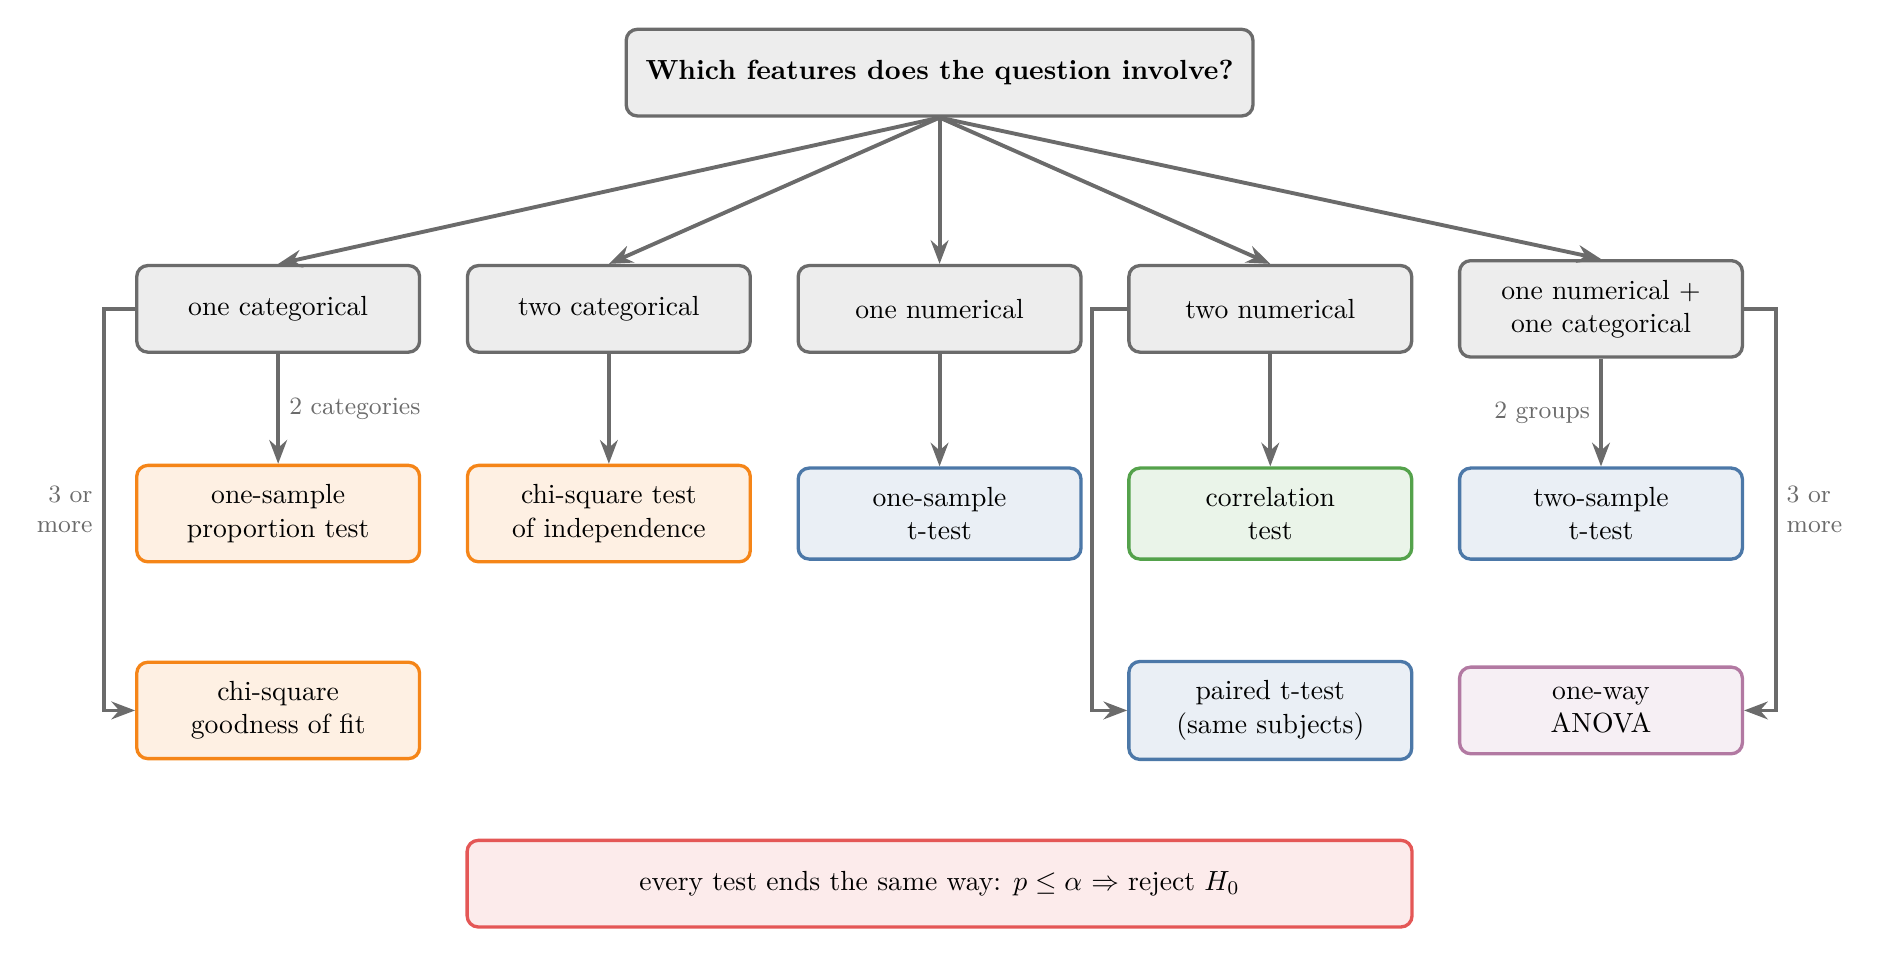
\begin{tikzpicture}[q/.style={box=cgrey, minimum width=3.3cm, text width=3.1cm},
                    t/.style={box=#1, minimum width=3.3cm, text width=3.1cm}, t/.default=cblue]
  \node[box=cgrey, minimum width=6cm] (root) at (8.4,3) {\textbf{Which features does the question involve?}};
  % the five kinds of question
  \node[q] (c1) at (0,0)    {one categorical};
  \node[q] (c2) at (4.2,0)  {two categorical};
  \node[q] (n1) at (8.4,0)  {one numerical};
  \node[q] (n2) at (12.6,0) {two numerical};
  \node[q] (nc) at (16.8,0) {one numerical +\\ one categorical};
  \foreach \n in {c1,c2,n1,n2,nc} \draw[arrow] (root.south) -- (\n.north);
  % tests
  \node[t=corange] (prop) at (0,-2.6)   {one-sample\\ proportion test};
  \node[t=corange] (gof) at (0,-5.1)    {chi-square\\ goodness of fit};
  \node[t=corange] (ind) at (4.2,-2.6)  {chi-square test\\ of independence};
  \node[t=cblue] (t1) at (8.4,-2.6)     {one-sample\\ t-test};
  \node[t=cgreen] (cor) at (12.6,-2.6)  {correlation\\ test};
  \node[t=cblue] (t2) at (16.8,-2.6)    {two-sample\\ t-test};
  \node[t=cblue] (pt) at (12.6,-5.1)   {paired t-test\\ (same subjects)};
  \node[t=cpurple] (an) at (16.8,-5.1)  {one-way\\ ANOVA};
  \foreach \a/\b in {c2/ind,n1/t1,n2/cor} \draw[arrow] (\a) -- (\b);
  \draw[arrow] (c1) -- (prop) node[midway, right, note] {2 categories};
  \draw[arrow] (n2.west) -- ++(-0.45,0) |- (pt.west);
  \draw[arrow] (nc) -- (t2) node[midway, left, note] {2 groups};
  \draw[arrow] (c1.west) -- ++(-0.4,0) |- (gof.west) node[pos=0.25, left, note, align=right] {3 or\\ more};
  \draw[arrow] (nc.east) -- ++(0.4,0) |- (an.east) node[pos=0.25, right, note, align=left] {3 or\\ more};
  % one decision rule for all
  \node[box=cred, minimum width=12cm] (rule) at (8.4,-7.3) {every test ends the same way: $p \le \alpha$ $\Rightarrow$ reject $H_0$};
\end{tikzpicture}
\end{document}
